\chapter{Teoretická část}


\section[Jednotné přijímací zkoušky pro střední školy a gymnázia]{Jednotné přijímací zkoušky\\pro střední školy a gymnázia}

Přijímací zkoušky tvoří příspěvková organizace CERMAT neboli Centrum pro zjišťování výsledků vzdělávání, která byla zřízena Ministerstvem školství, mládeže a tělovýchovy ČR v roce 2006.~\cite{zakon_CERMAT} Tato organizace také zařizuje státní maturitní zkoušky a závěrečné zkoušky.~\cite{CERMAT_p_m}



Jde o národně jednotné přijímací zkoušky, které jsou povinnou součástí prvního kola přijímacího řízení do všech maturitních oborů s výjimkou oborů s talentovou zkouškou a oborů zkráceného studia.

„Jednotná přijímací zkouška se skládá ze dvou písemných testů - z českého jazyka a literatury a z matematiky.
Varianty testů jsou různé pro čtyřleté obory vzdělání (včetně oborů nástavbového studia), pro šestiletá gymnázia a pro osmiletá gymnázia.
Maximální možný počet dosažených bodů v testech z matematiky i českého jazyka a literatury je 50 bodů.”~\cite{CERMAT_co_to_je}

V České republice byly jednotné přijímací zkoušky testovány v letech 2015 a~2016, povinně zavedeny byly v roce 2017.~\cite{CERMAT_rocni_zprava}

Přijímací zkoušky z předchozích roků jsou dostupné na webových stránkách Centra pro zjišťování výsledků vzdělávání.~\cite{CERMAT_pdfka}


\section{Vysvětlení teoretických základů}

\subsection{Obvod}
Obvod je součet délek čar, které vymezují nějaký útvar.~\cite{umim_mat}

\begin{figure}[h]
    \centering
    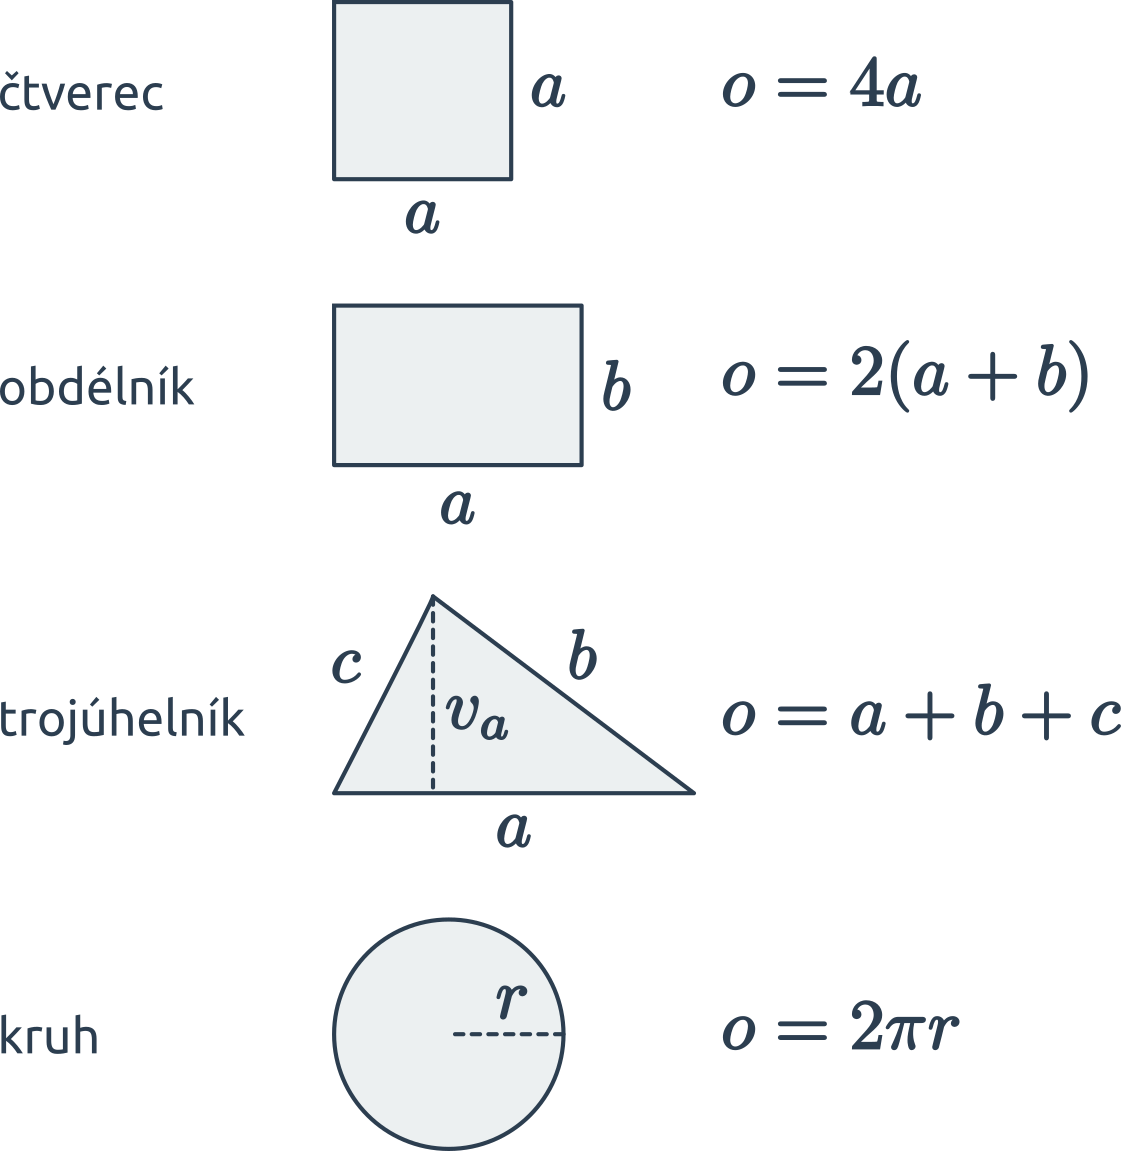
\includegraphics[width=0.6\textwidth]{teor/obvod}
    \caption{Vzorce pro výpočet obvodu~\cite{umim_mat}}
\end{figure}

Ve čtvercové síti lze obvod spočítat sečtením všech čar, které útvar tvoří. Pokud čáry nevedou rovnoběžně se sítí, můžeme je i přesto odečítat.

\subsubsection{Příklad}
\begin{minipage}[t]{\linewidth}
    Pokud chceme znát rozdíl obvodů těchto dvou tvarů, nemusíme znát oba dva obvody. U obou tvarů neznáme délku čáry, která není rovnoběžná se sítí. Víme ale, že jsou stejně dlouhé. Můžeme je tedy odečíst a pak počítat s rozdíly zbytku, které dokážeme jednoduše určit.

    Pokud je délka strany čtverce, ze kterého je čtvercové pole 1 cm, rozdíl obvodů jsou 2 cm.
    \begin{center}
        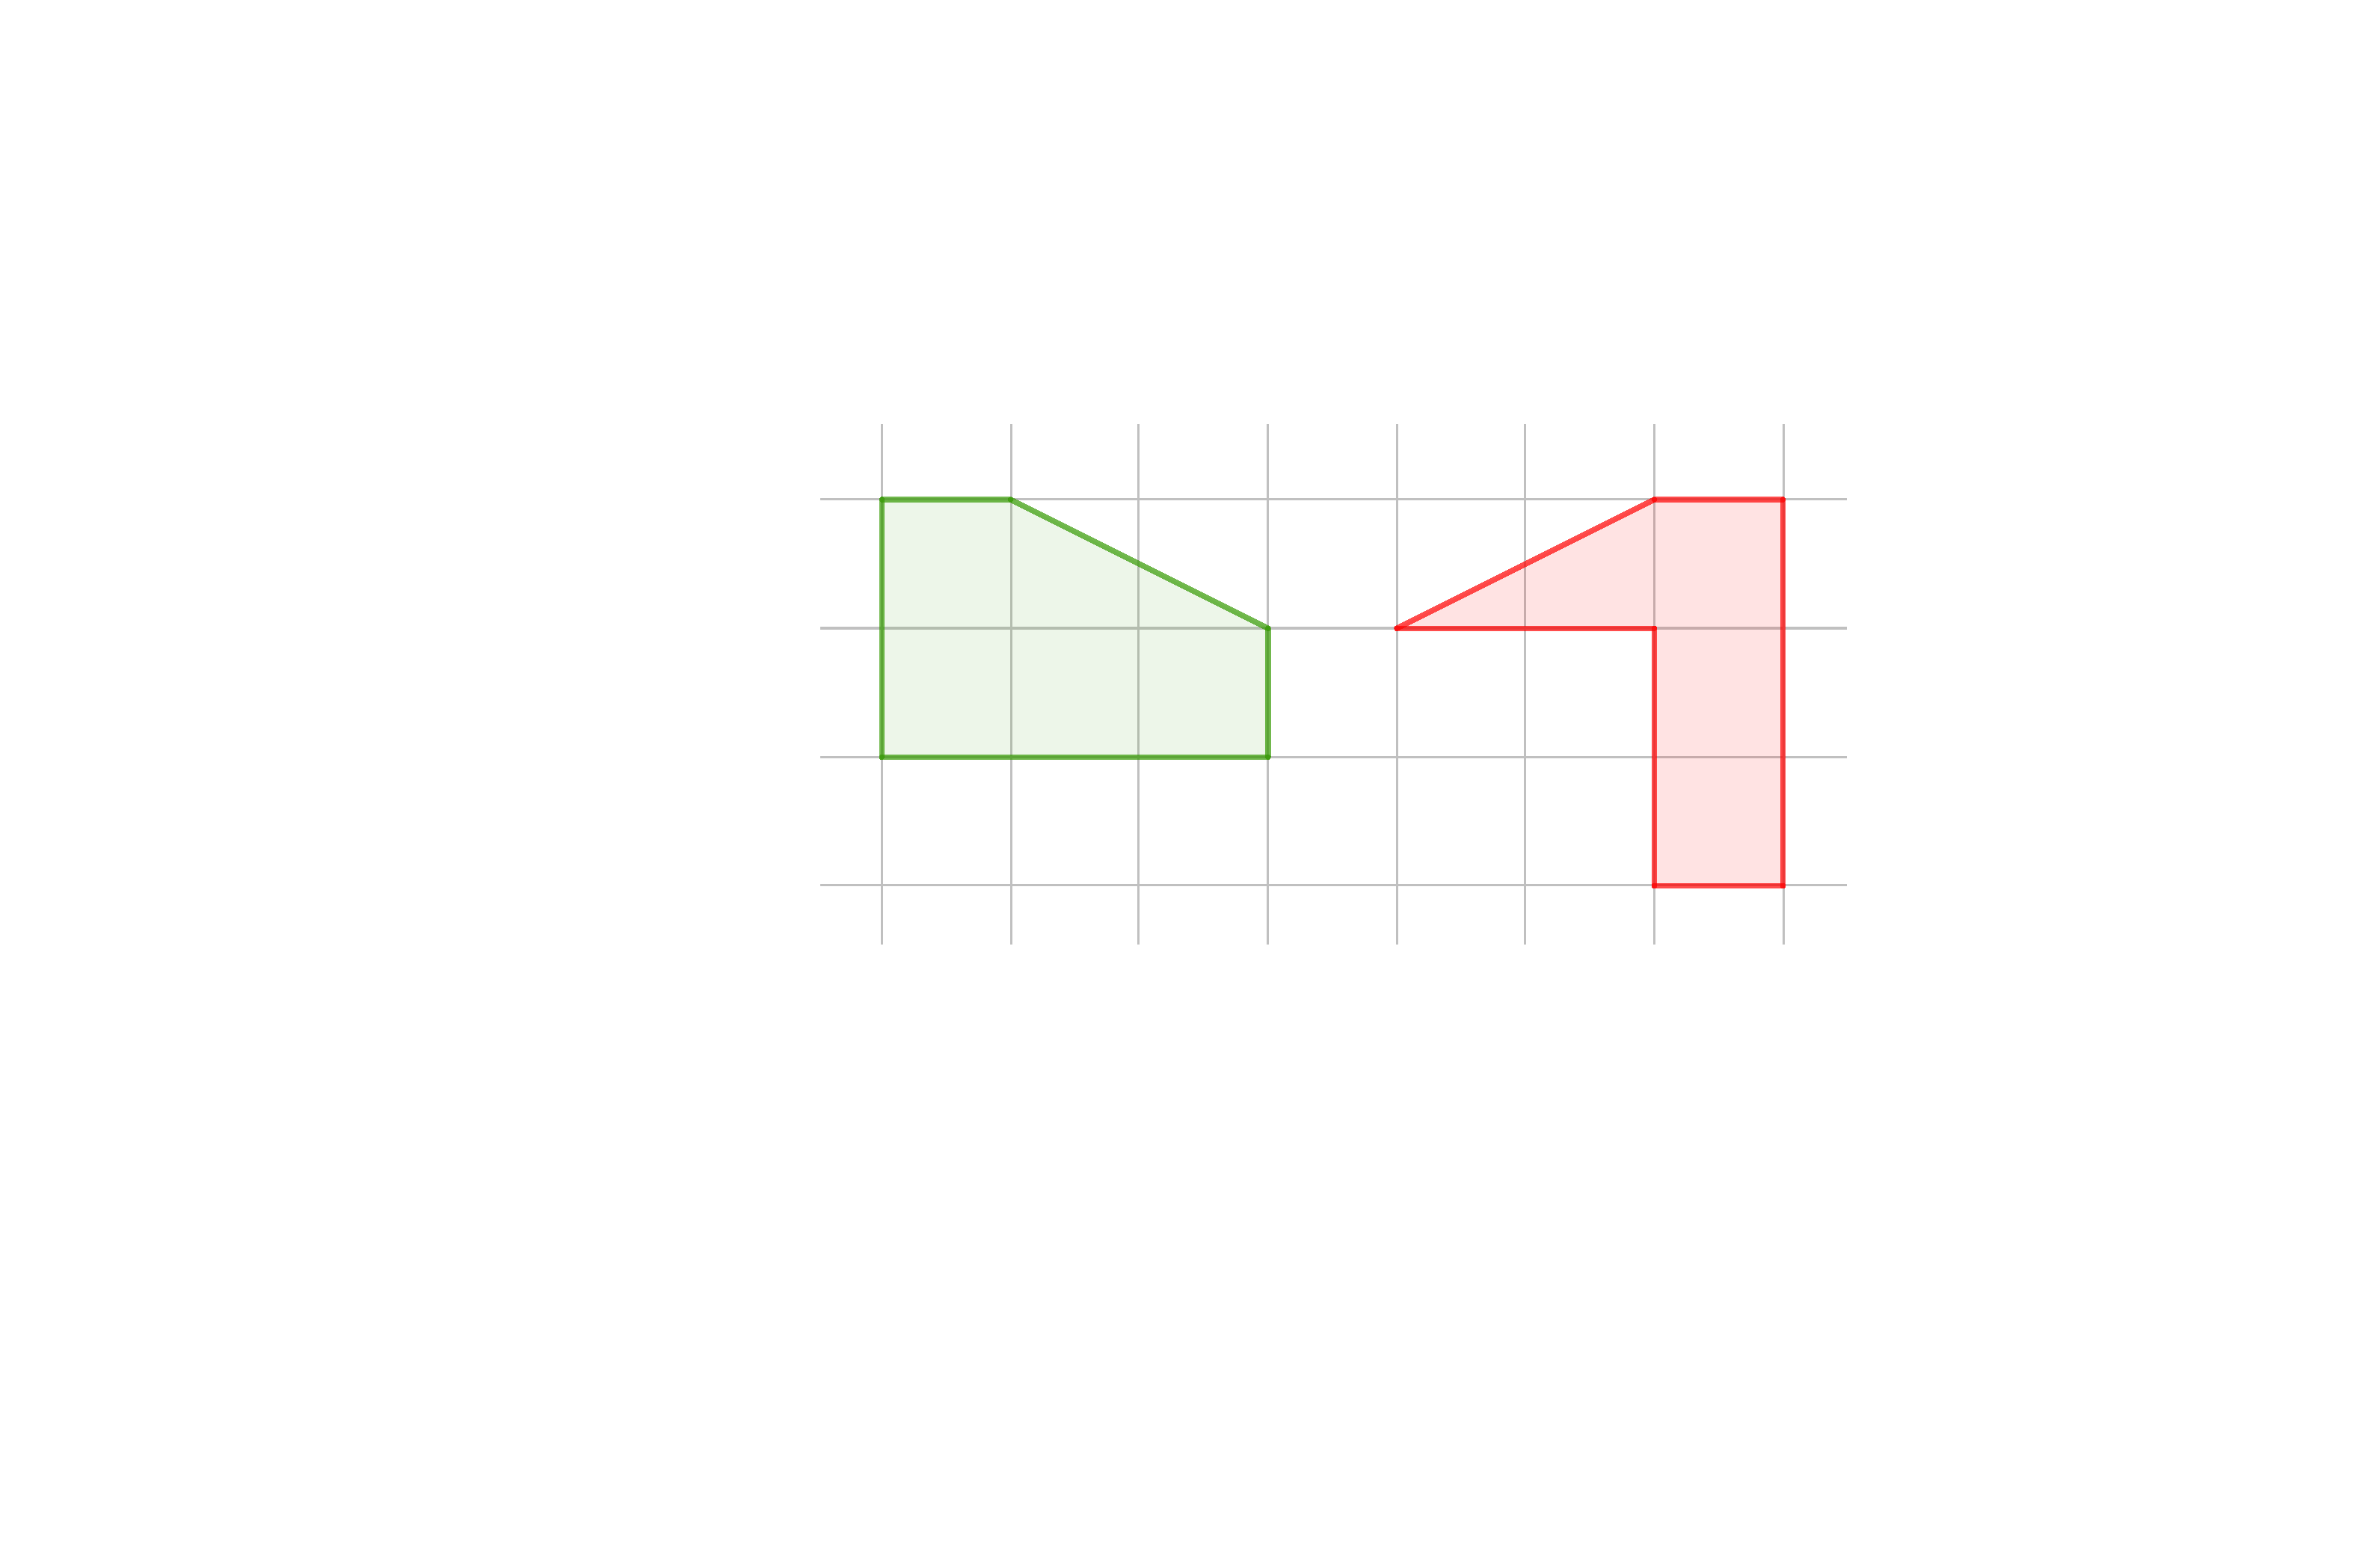
\includegraphics[width=0.6\textwidth]{teor/priklad-obvod}
    \end{center}
\end{minipage}

\subsection{Obsah}
Obsah vyjadřuje, kolik „místa v rovině“ útvar zaujímá. Měří se v jednotkách obsahu.~\cite{umim_mat}

Příkladem jednotek obsahu jsou centimetry čtvereční ($\text{cm}^{2}$) nebo metry čtvereční ($\text{m}^{2}$).



K výpočtu obsahu je nejdůležitější pamatovat si vzorce. Pokud je útvar složitý, budeme jich muset použít několik.

\begin{figure}[h]
	\centering
	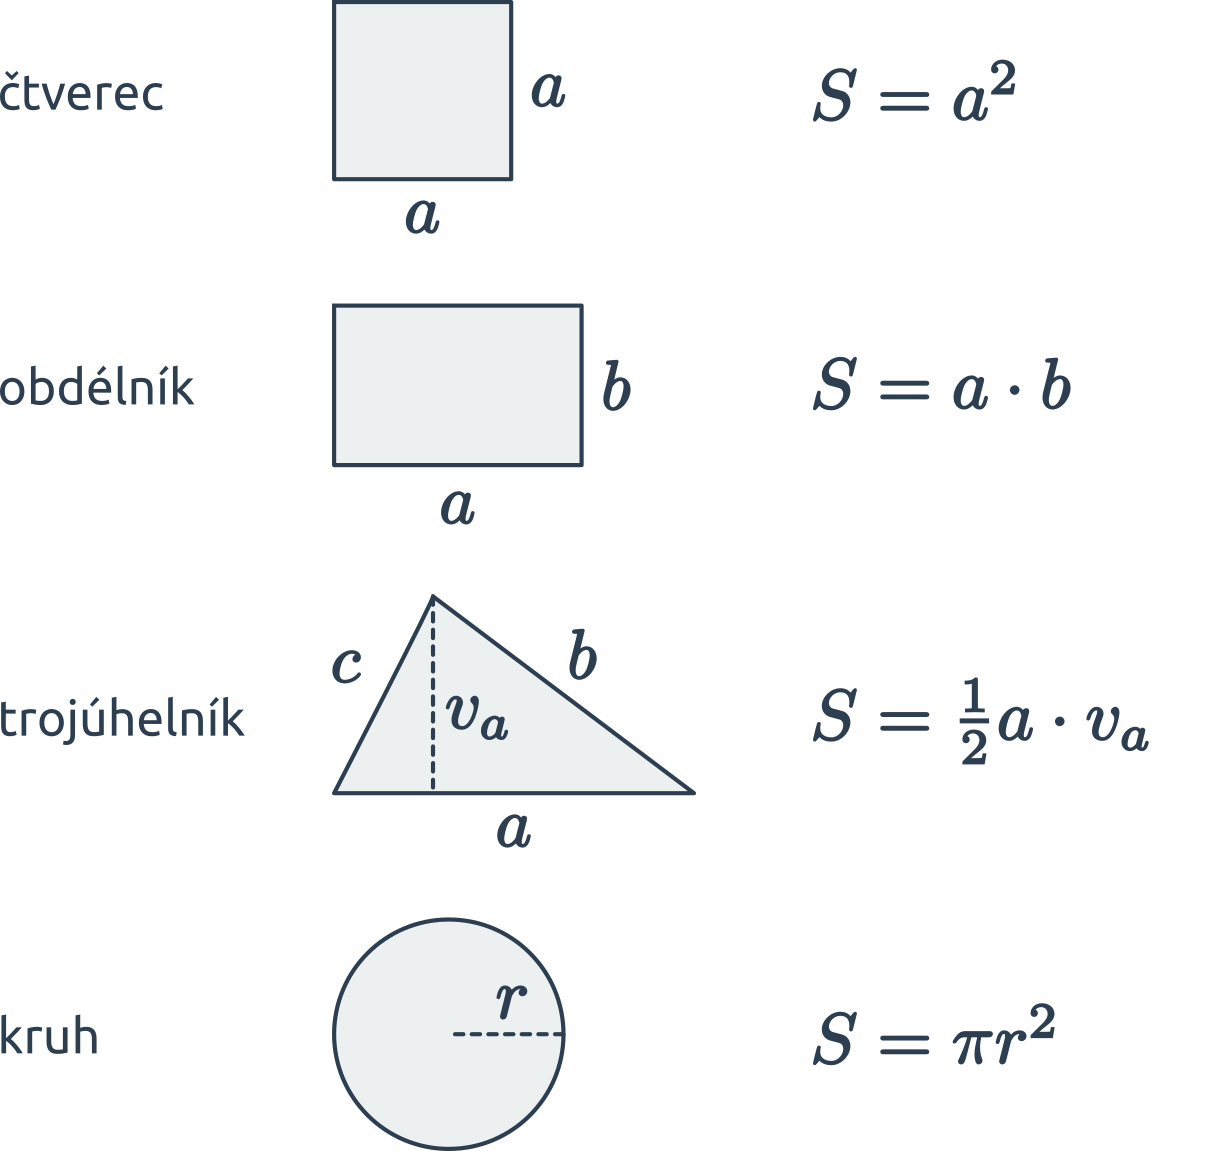
\includegraphics[width=0.6\textwidth]{teor/obsah}
	\caption{Vzorce pro výpočet obsahu~\cite{umim_mat}}
\end{figure}

\subsubsection{Příklad}
\begin{minipage}[t]{\linewidth}
    Pokud potřebujeme vypočítat obsah tvaru ABCD, stačí si uvědomit, že ho můžeme vypočítat jako obsah velkého (zeleného) trojúhelníku mínus obsah menšího (růžového) trojúhelníku.

    $ \frac{7\cdot4}{2} - \frac{3\cdot2}{2} =  14 - 3 = 11 \text{ cm}^{2}$.
    \begin{center}
        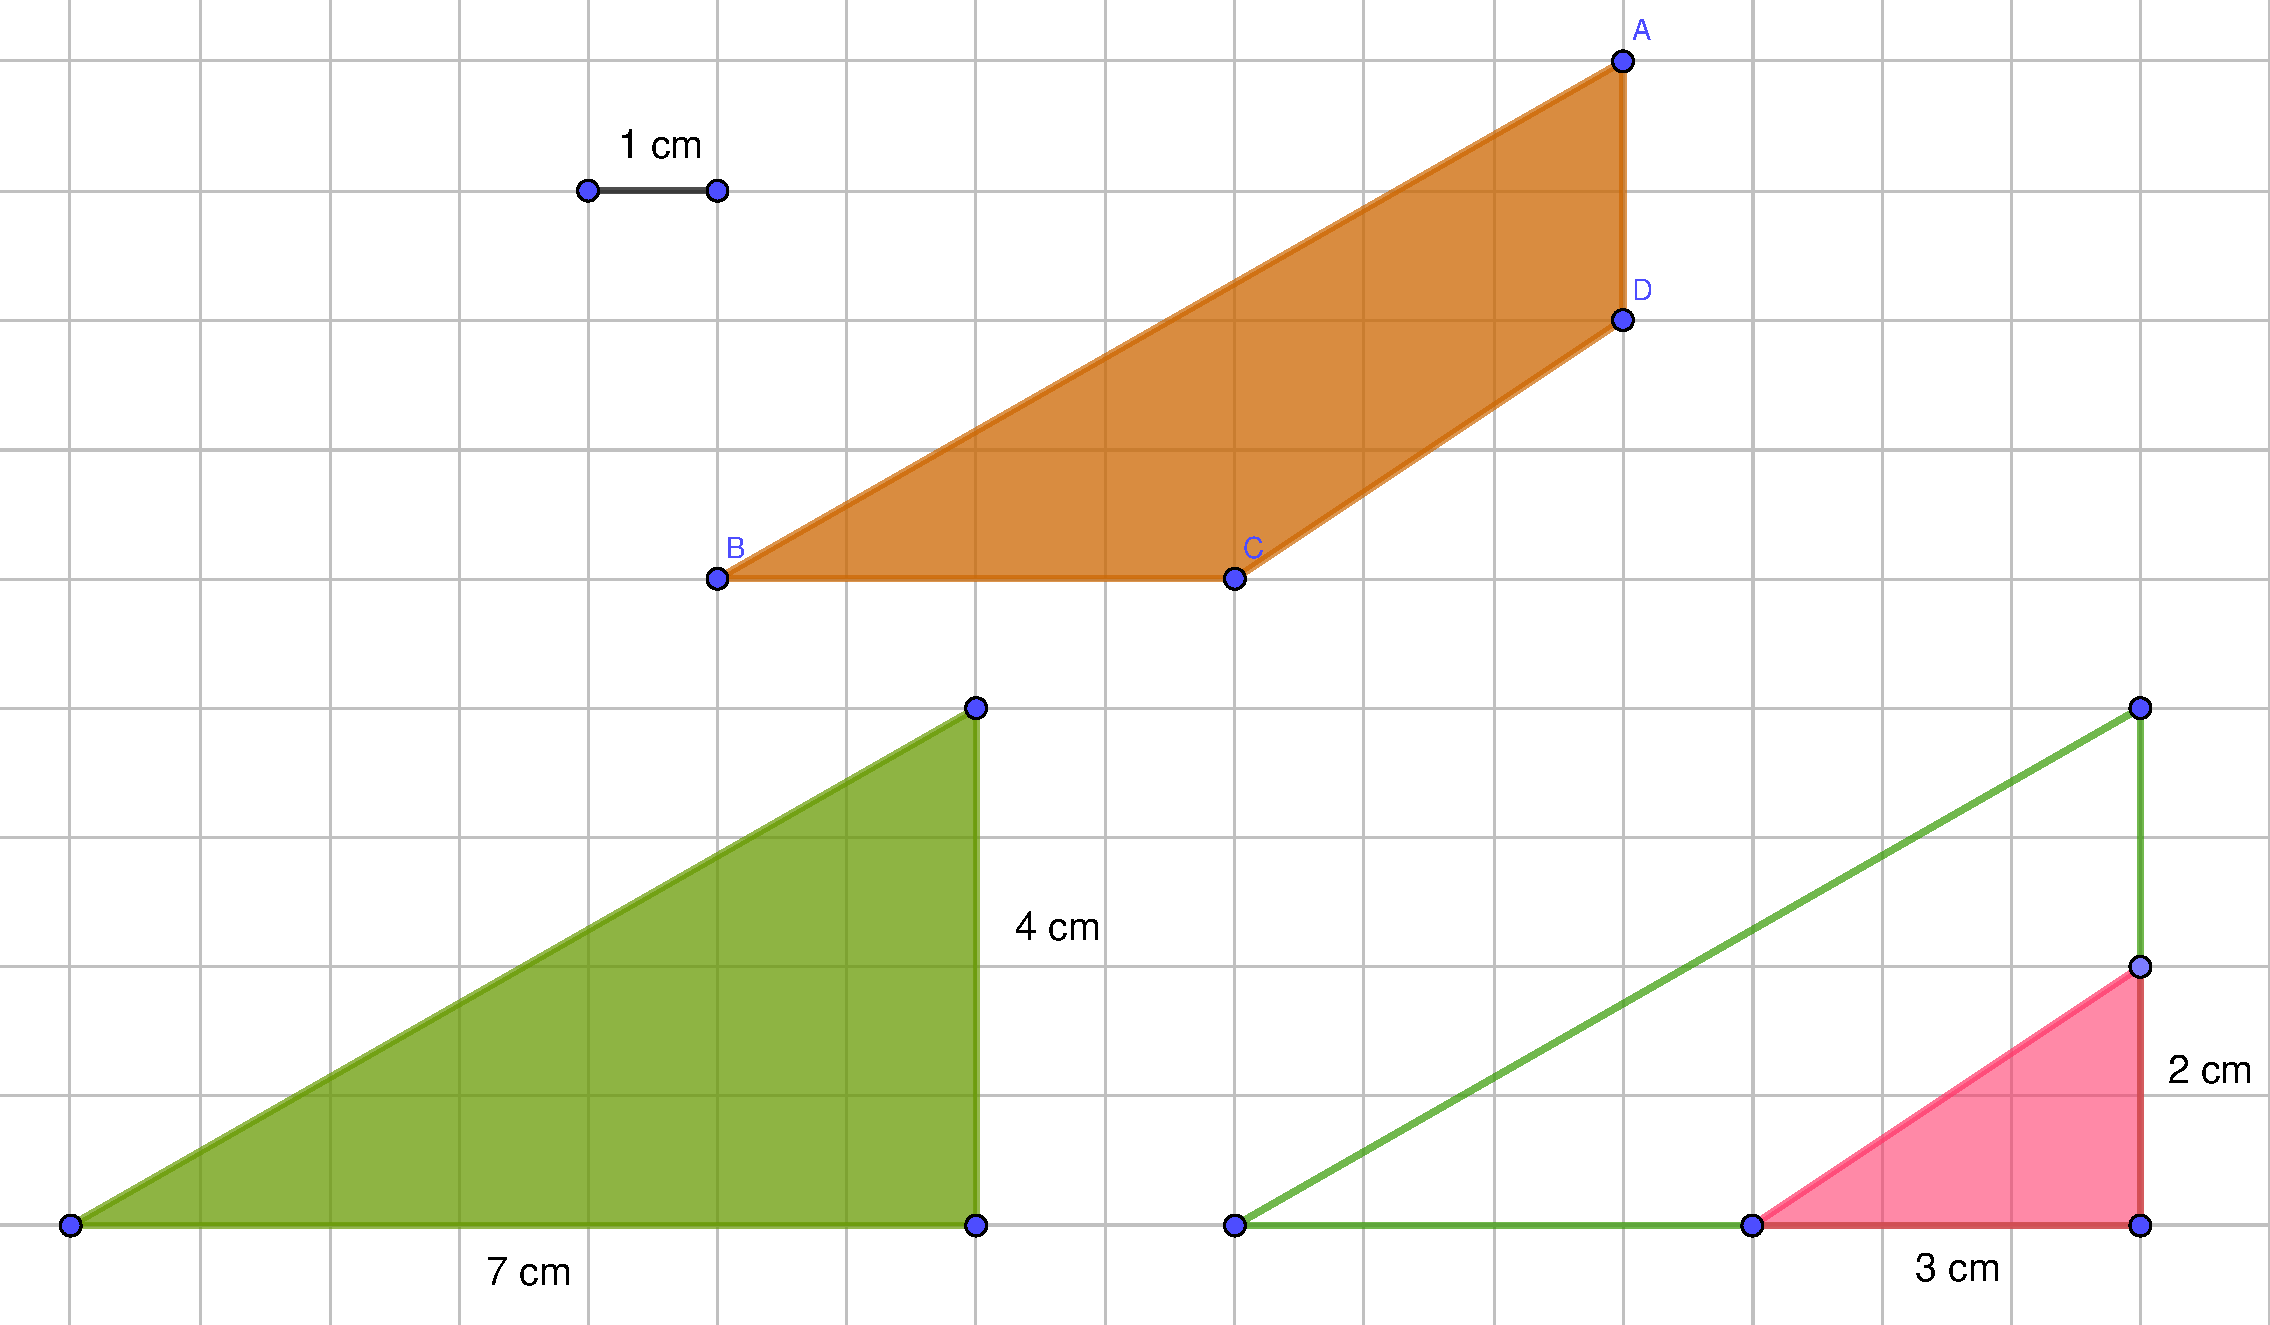
\includegraphics[width=0.6\textwidth]{teor/priklad-obsah}
    \end{center}
\end{minipage}

\subsection{Osová souměrnost}

Osová souměrnost je geometrické zobrazení. Při ní se každý bod útvaru zobrazí na druhou stranu nějaké předem určené osy, která se nazývá osa souměrnosti. Osa souměrnosti je určena přímkou.

Osová souměrnost se dá představit jako překlopení podle osy.

\subsubsection{Příklad}
\begin{minipage}[t]{\linewidth}
    Tyto dva trojúhelníky jsou osově souměrné, jelikož všechny jejich body jsou „překlopené” podle osy s.
    \begin{center}
        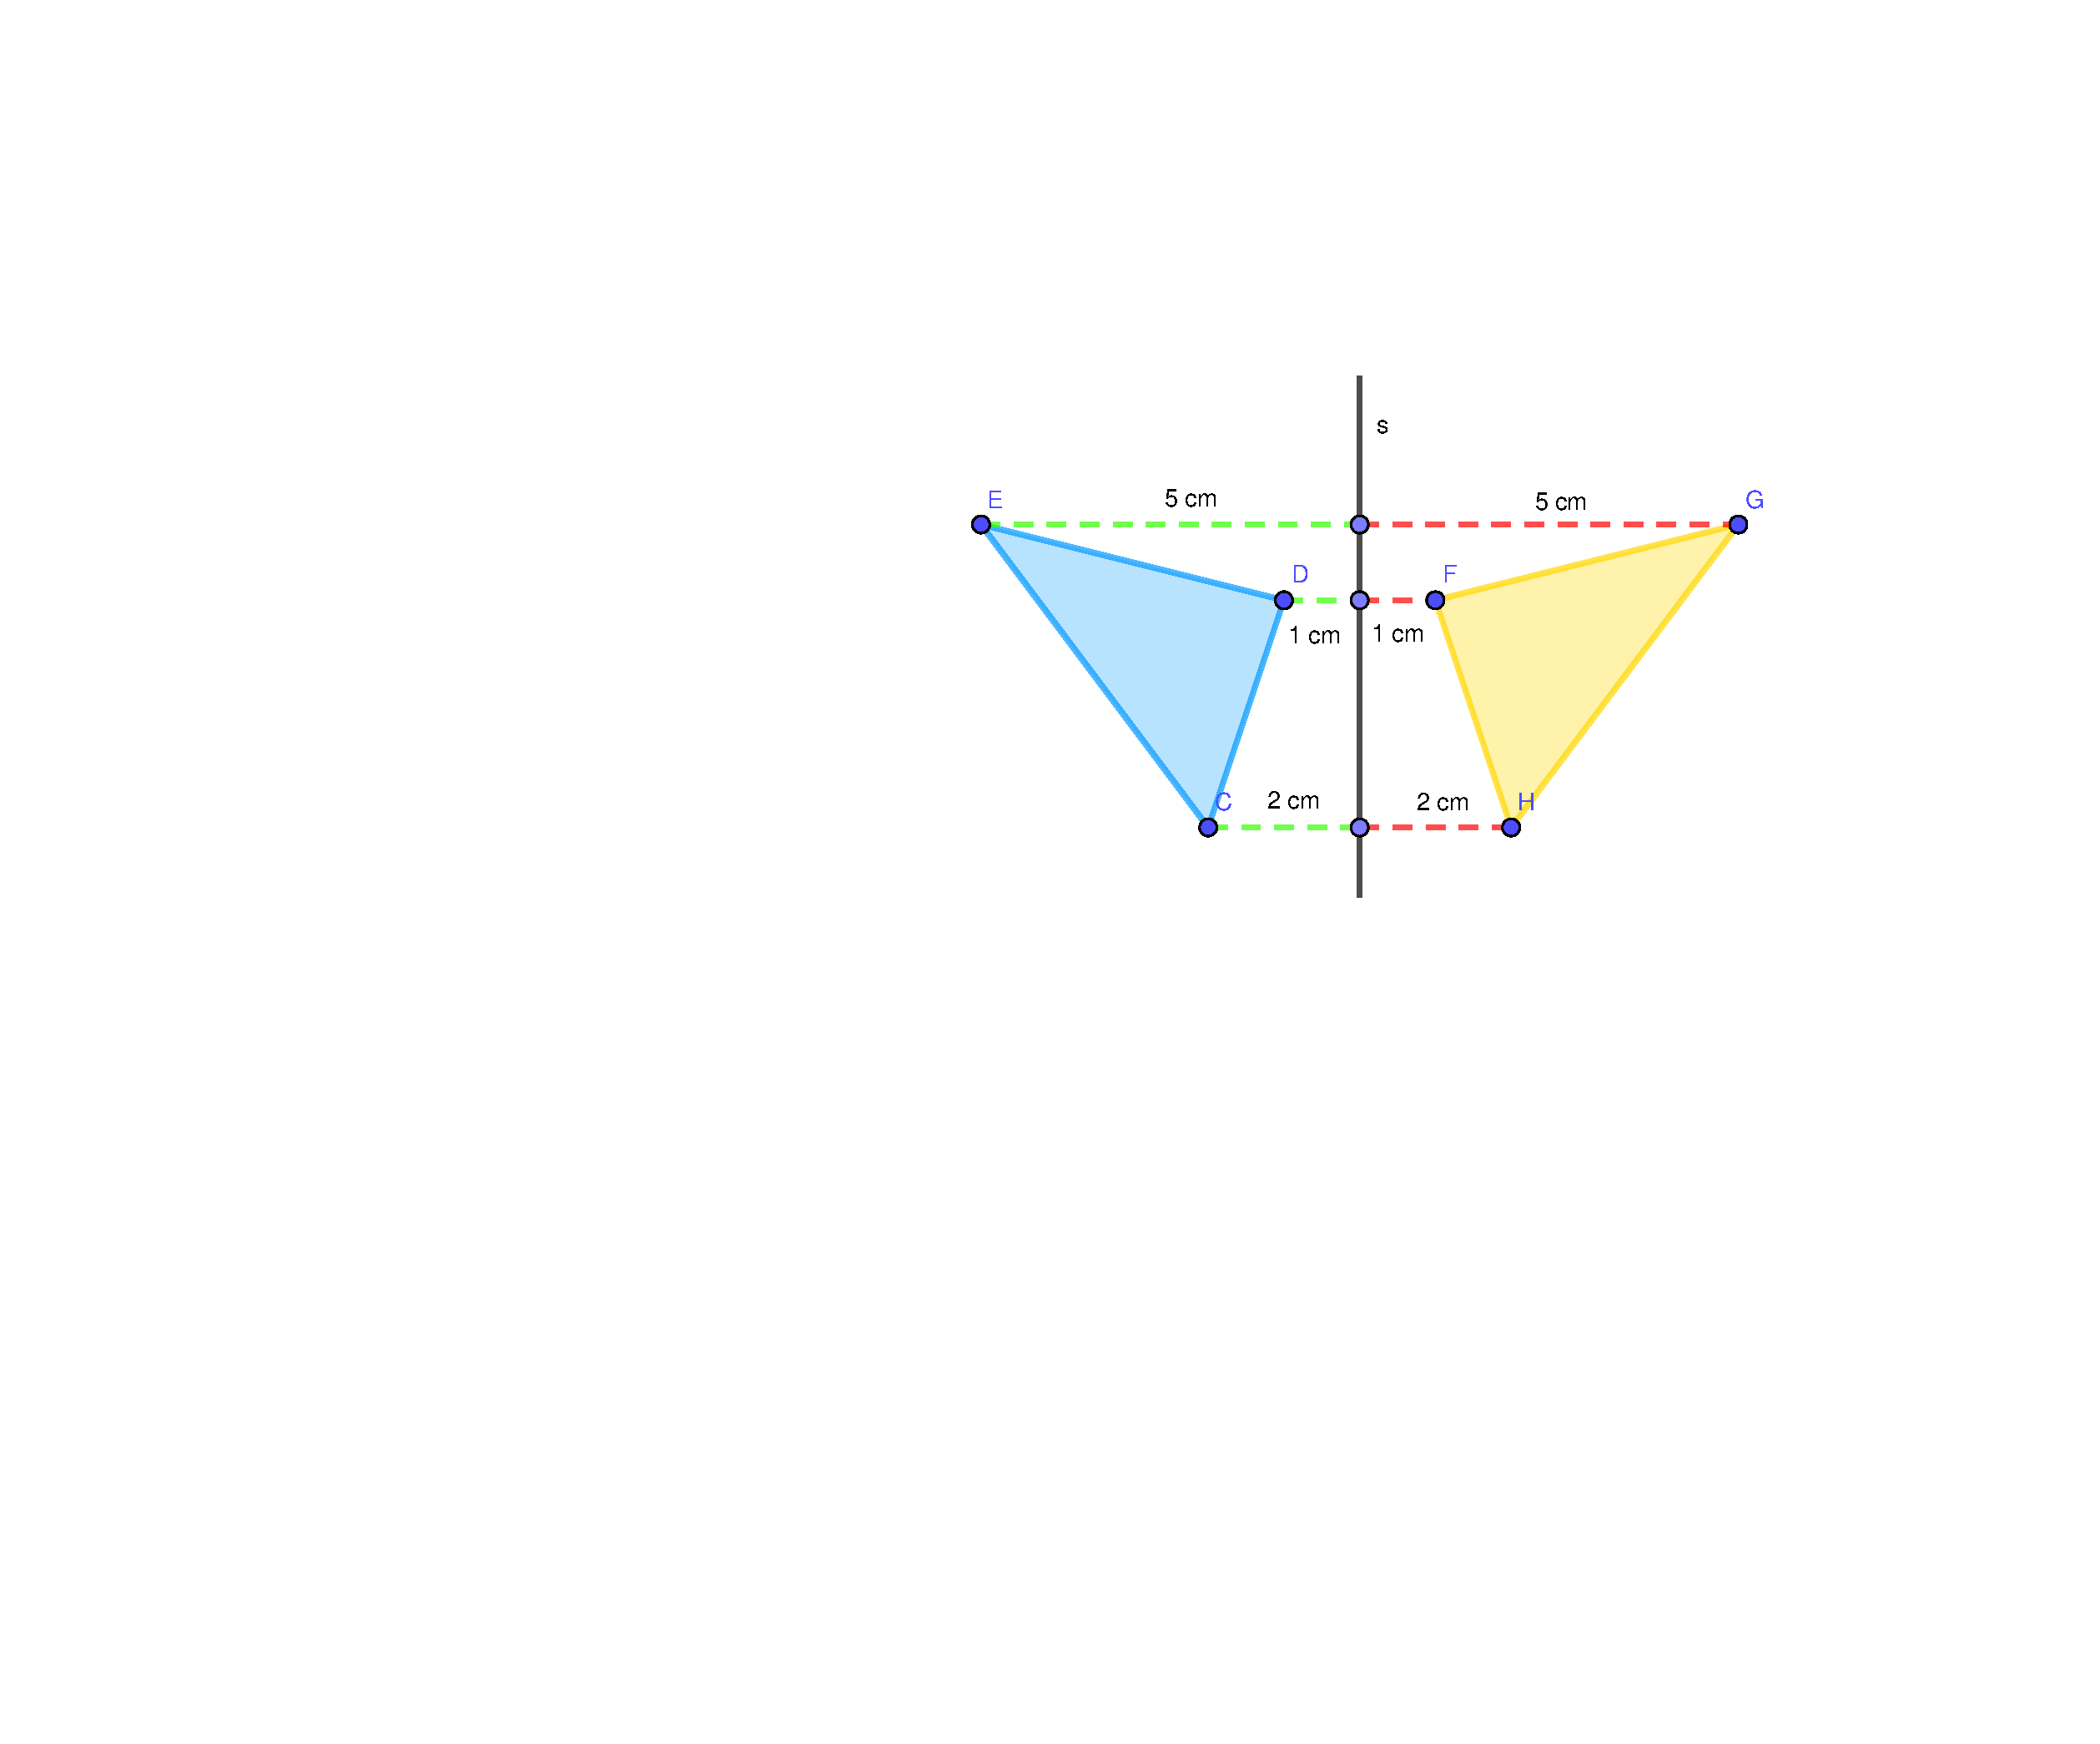
\includegraphics[width=0.6\textwidth]{teor/priklad-soum}
    \end{center}
\end{minipage}

\subsection{Rovnostranný trojúhelník}
Rovnostranný trojúhelník je trojúhelník, jehož všechny strany mají stejnou délku.

\begin{figure}[h]
    \centering
    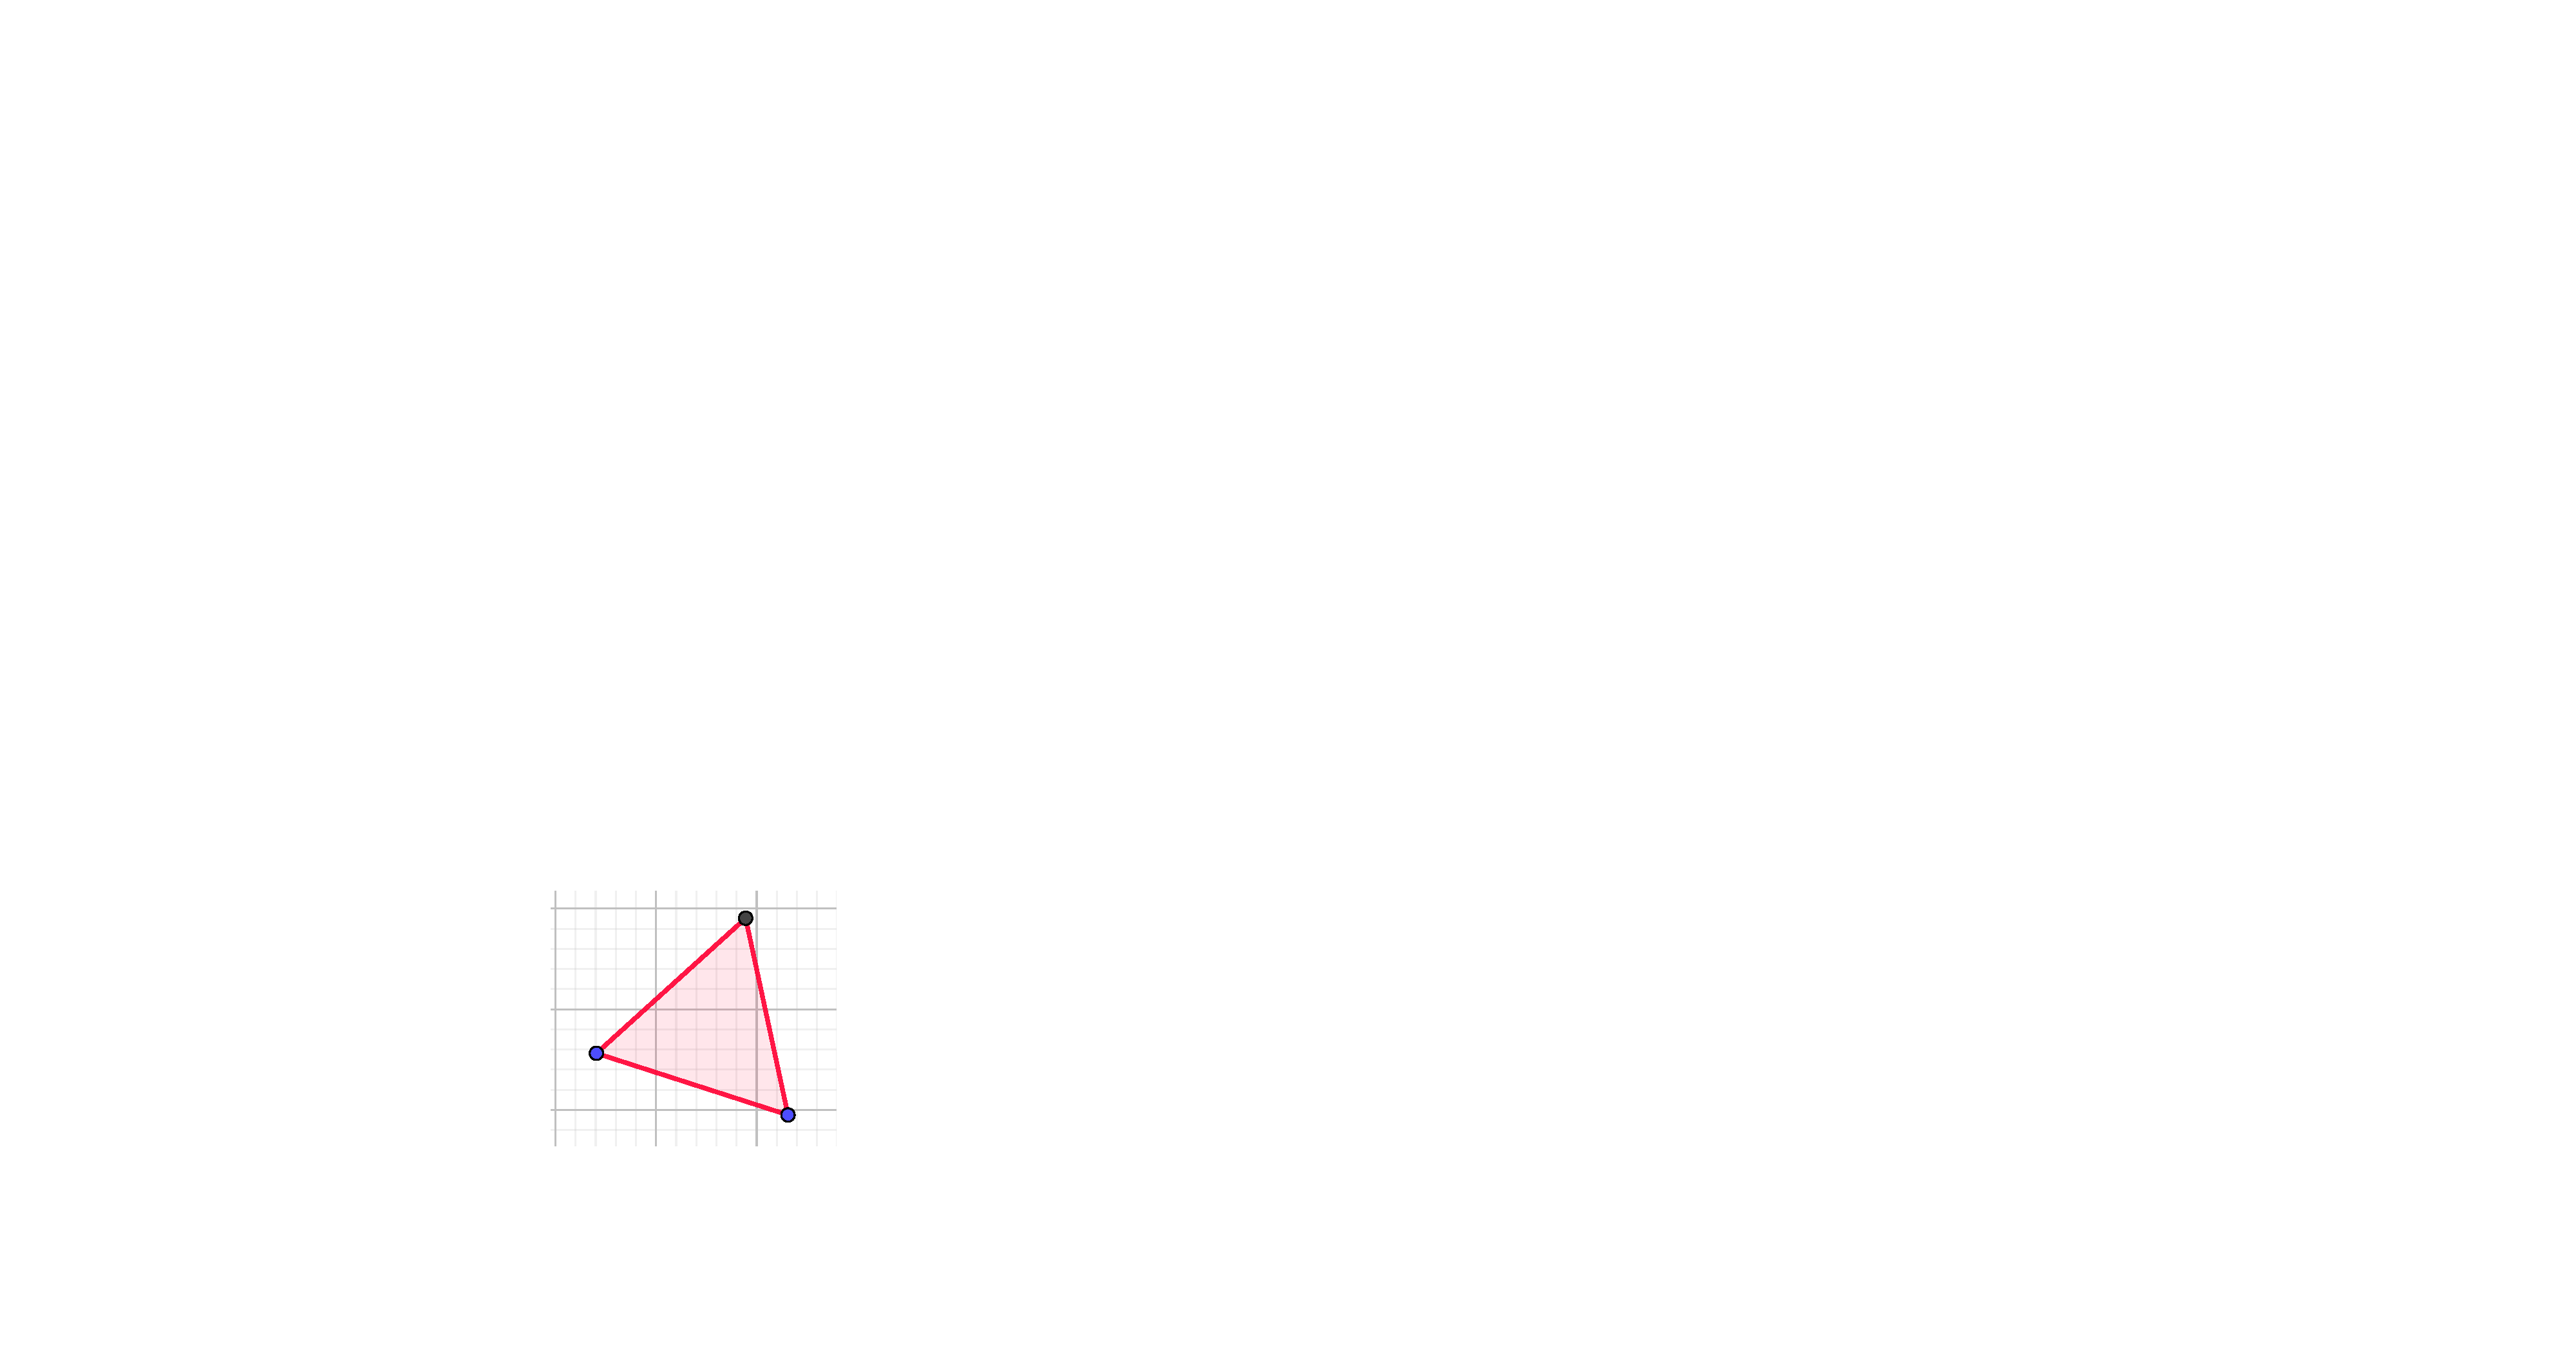
\includegraphics[width=0.3\textwidth]{teor/rovnostranny}
    \caption{Rovnostranný trojúhelník}
\end{figure}

\subsection{Rovnoramenný trojúhelník}
Rovnoramenný trojúhelník je trojúhelník, jehož dvě strany mají stejnou délku. Tyto dvě strany se nazývají ramena, třetí strana se jmenuje základna.

\begin{figure}[h]
    \centering
    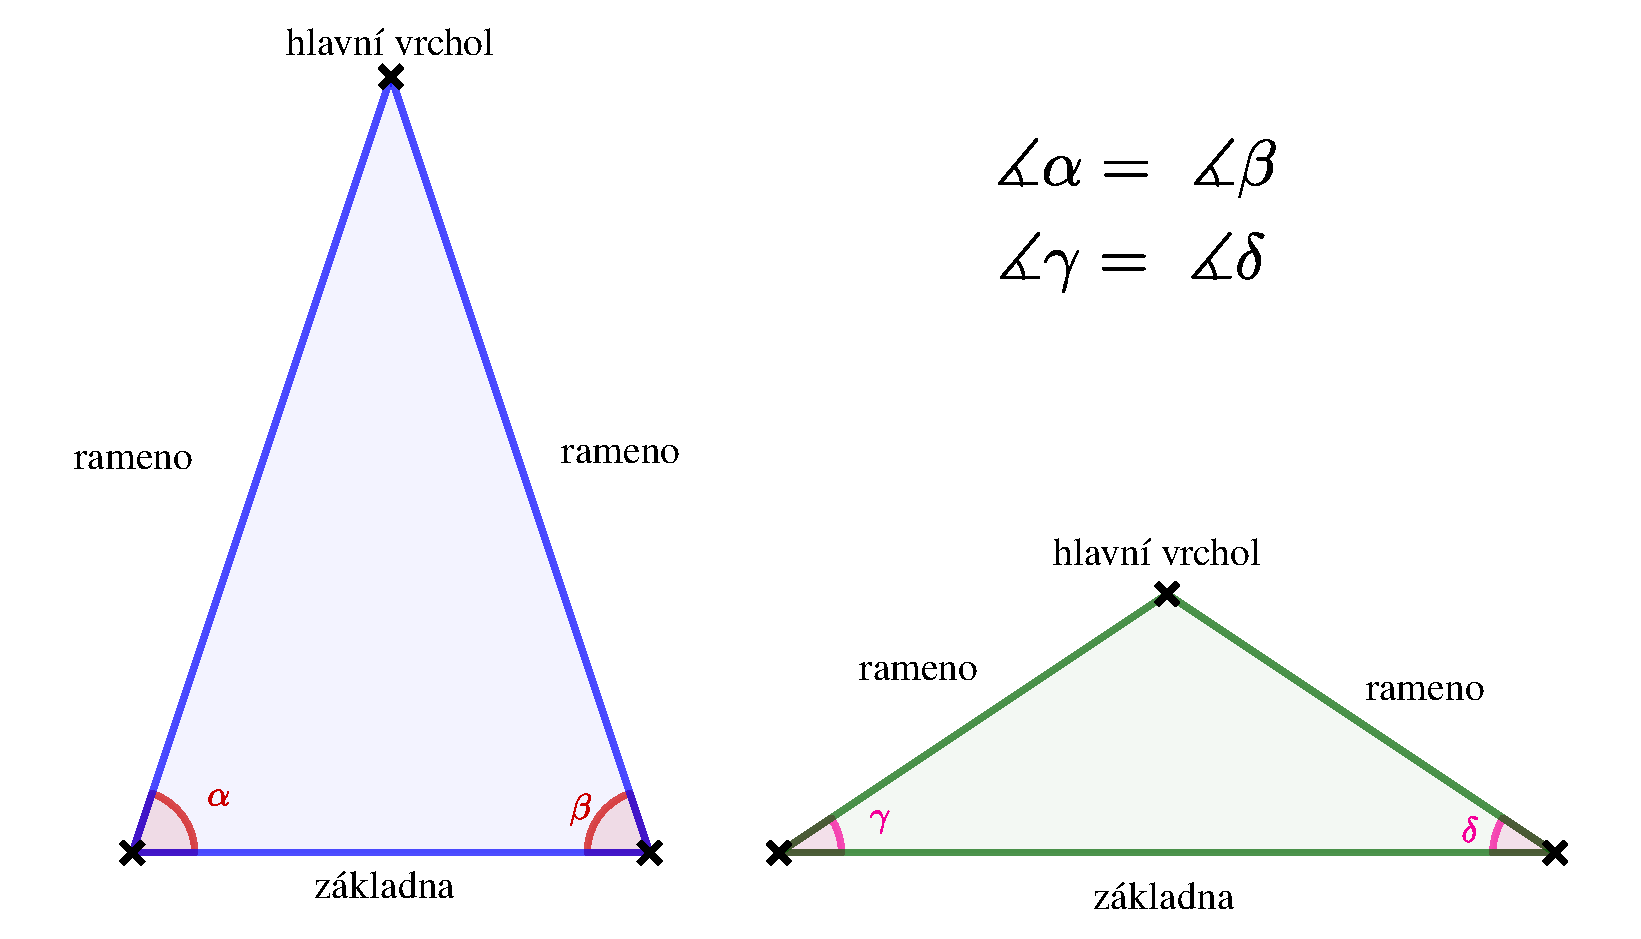
\includegraphics[width=0.6\textwidth]{teor/rovnoramenny}
    \caption{2 rovnoramenné trojúhelníky}
\end{figure}

\subsection{Shodnost trojúhelníků}
Dva trojúhelníky jsou navzájem shodné, pokud se rovnají délky všech jejich stran.

\subsection{Průsečík}
Průsečík je bod, ve kterém se protínají 2 čáry, například přímky nebo úsečky.

\begin{figure}[h]
    \centering
    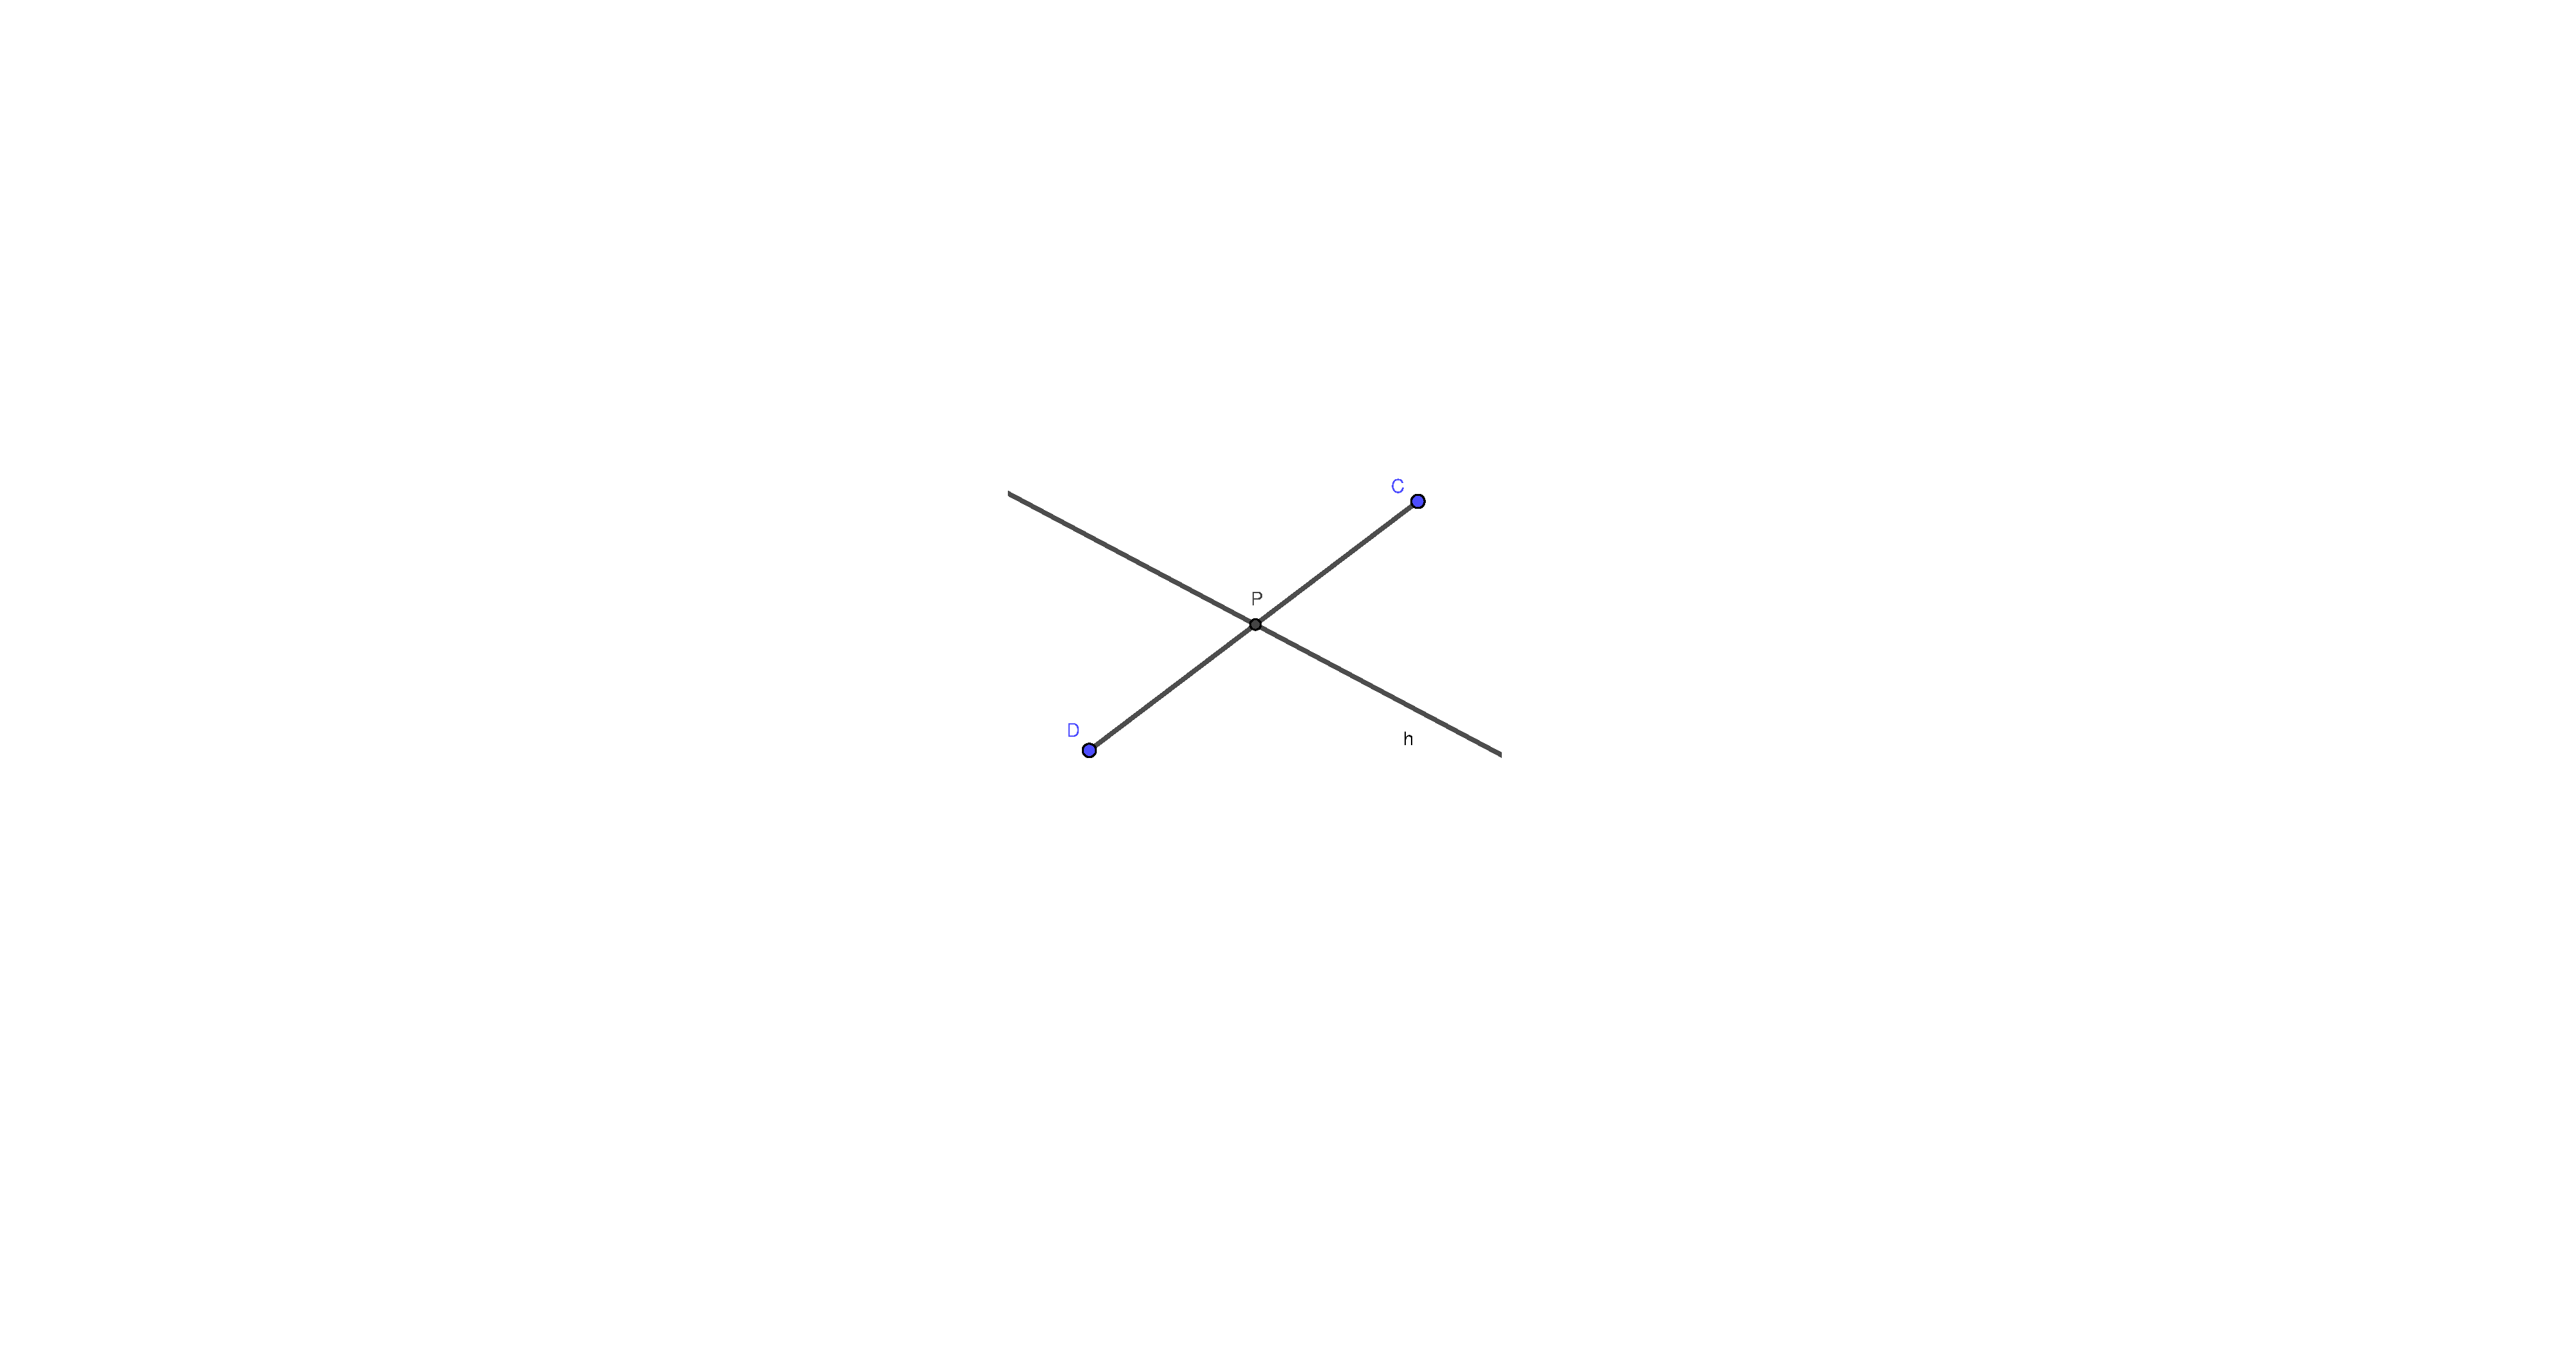
\includegraphics[width=0.6\textwidth]{teor/prusecik}
    \caption{Průsečík přímky h a úsečky CD, který je nazvaný P}
\end{figure}

\subsection{Pravý úhel, kolmost}
Pravý úhel je úhel o velikosti 90°. 2 čáry jsou na sebe kolmé, pokud svírají pravý úhel.

\begin{figure}[h]
    \centering
    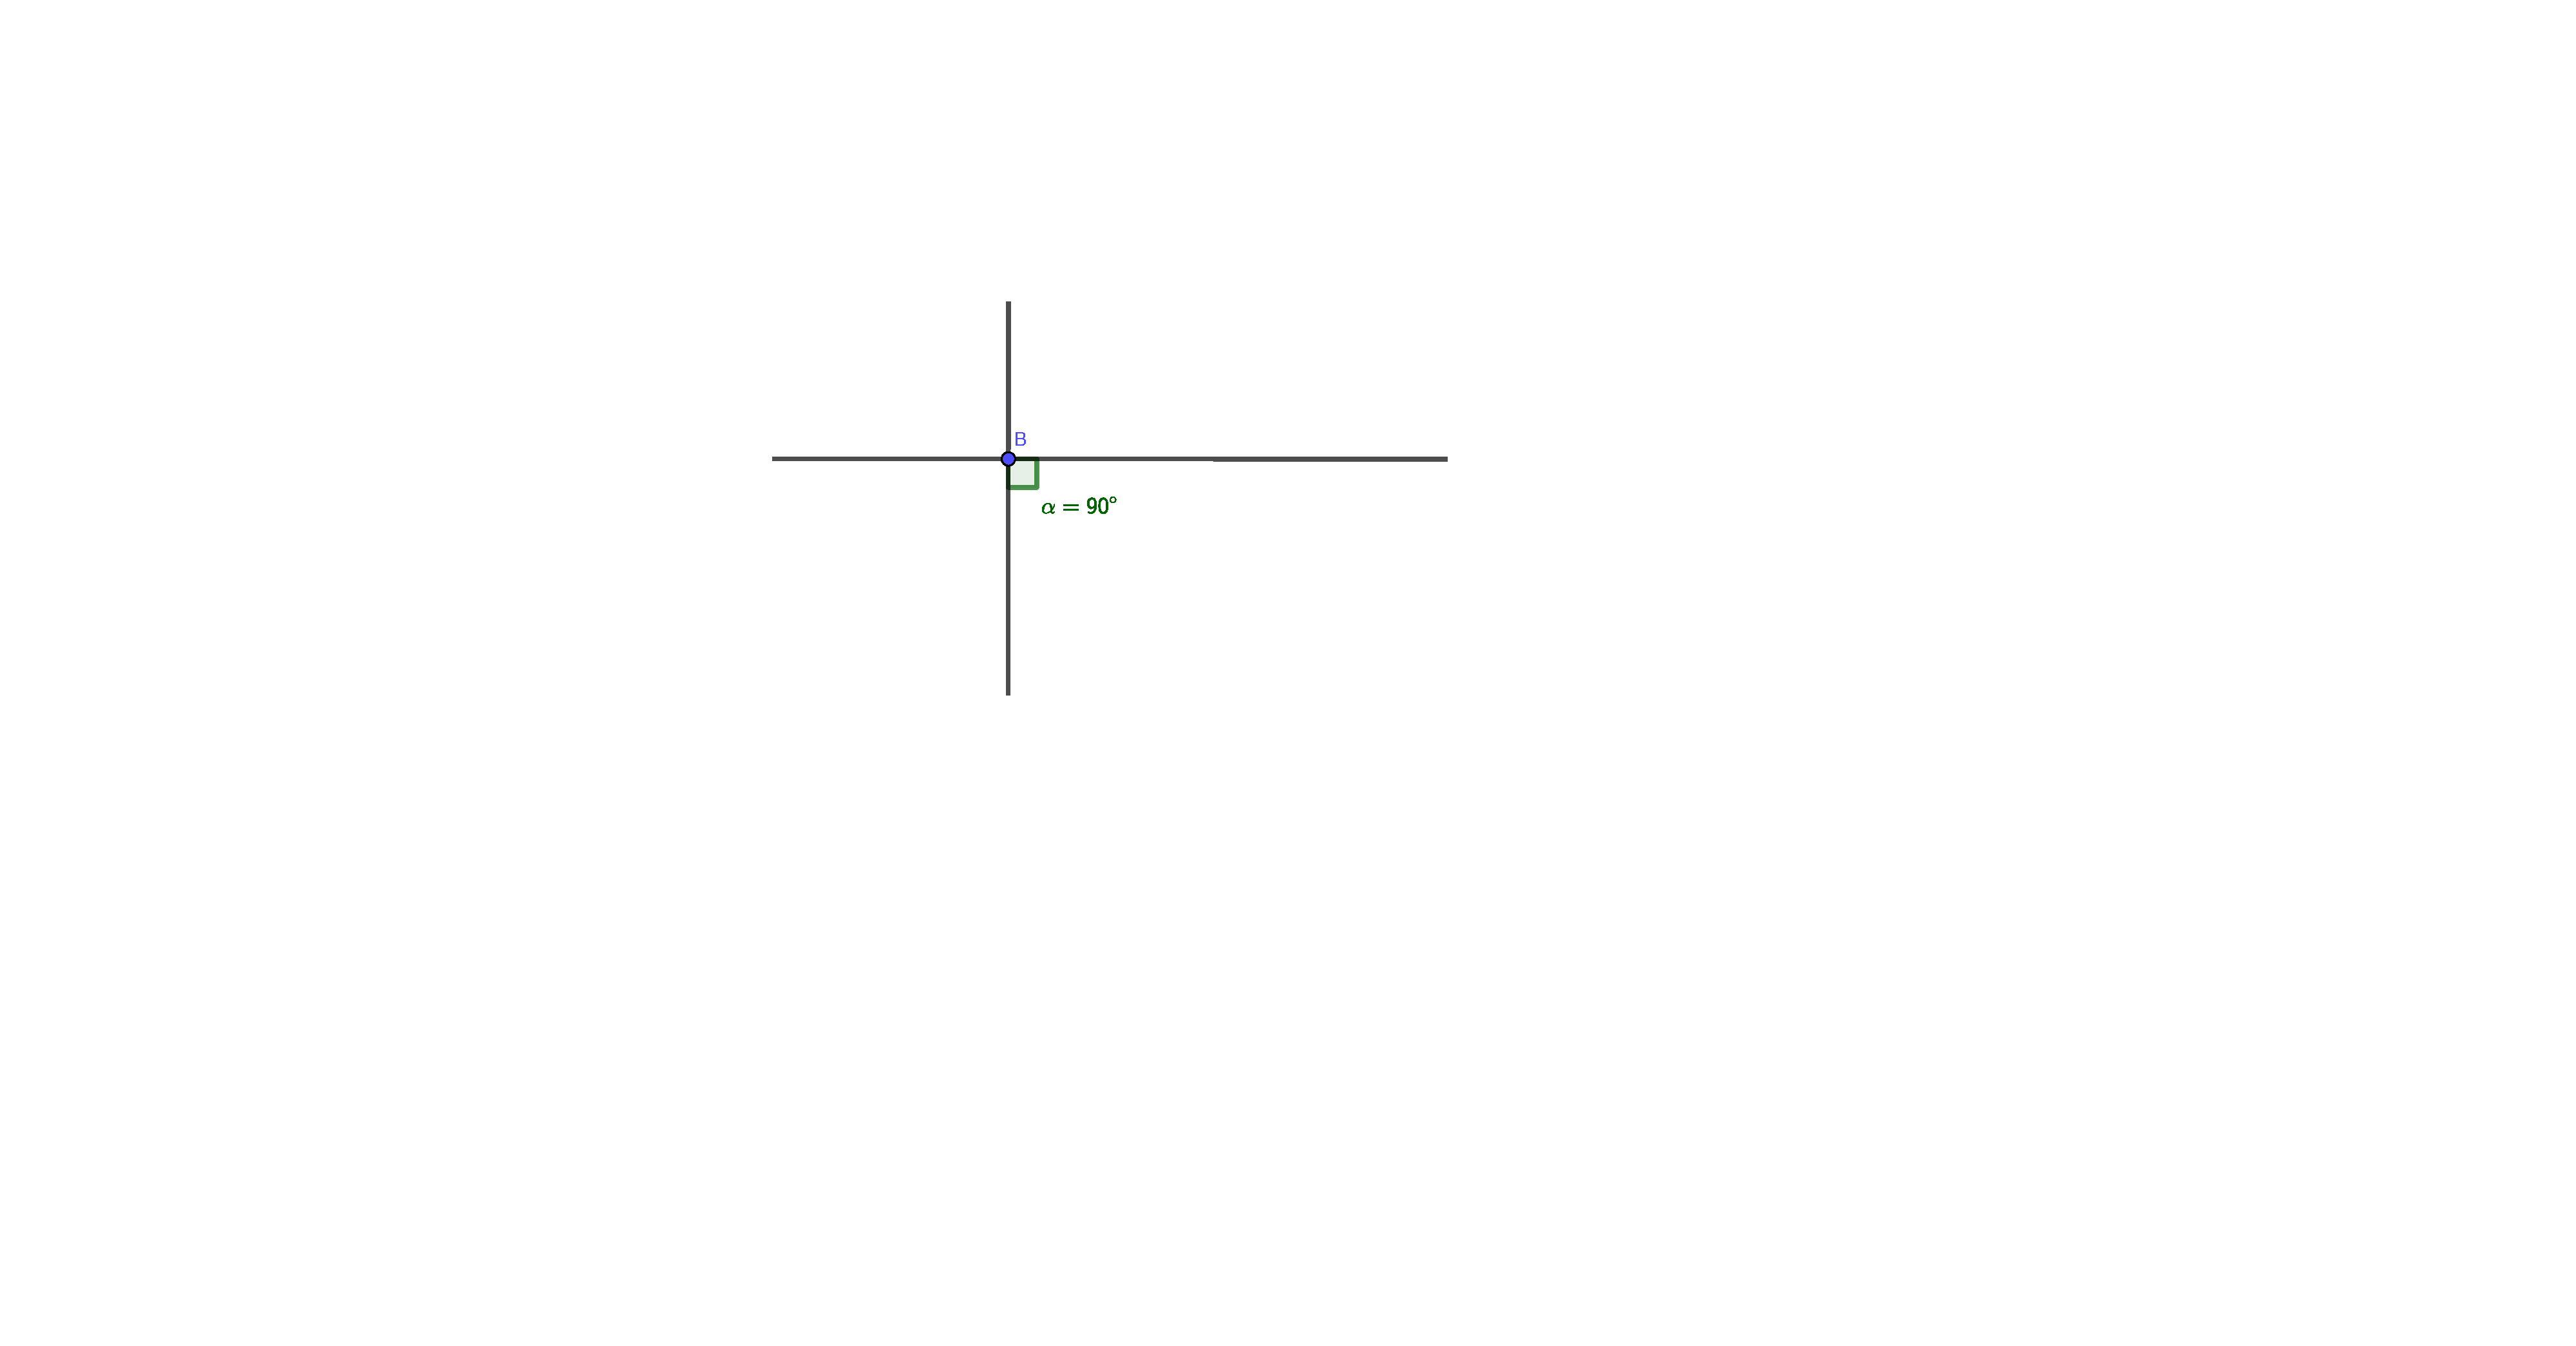
\includegraphics[width=0.4\textwidth]{teor/pravy-a-kolmo}
    \caption{Kolmice}
    \label{fig:kolm}
\end{figure}

Na obrázku~\ref{fig:kolm} jsou vidět 2 kolmé čáry svírající pravý úhel označený $\alpha$.

\subsection{Pravoúhlý trojúhelník}
Trojúhelník je pravoúhlý, pokud je jeden z jeho úhlů pravý.

\begin{figure}[h]
    \centering
    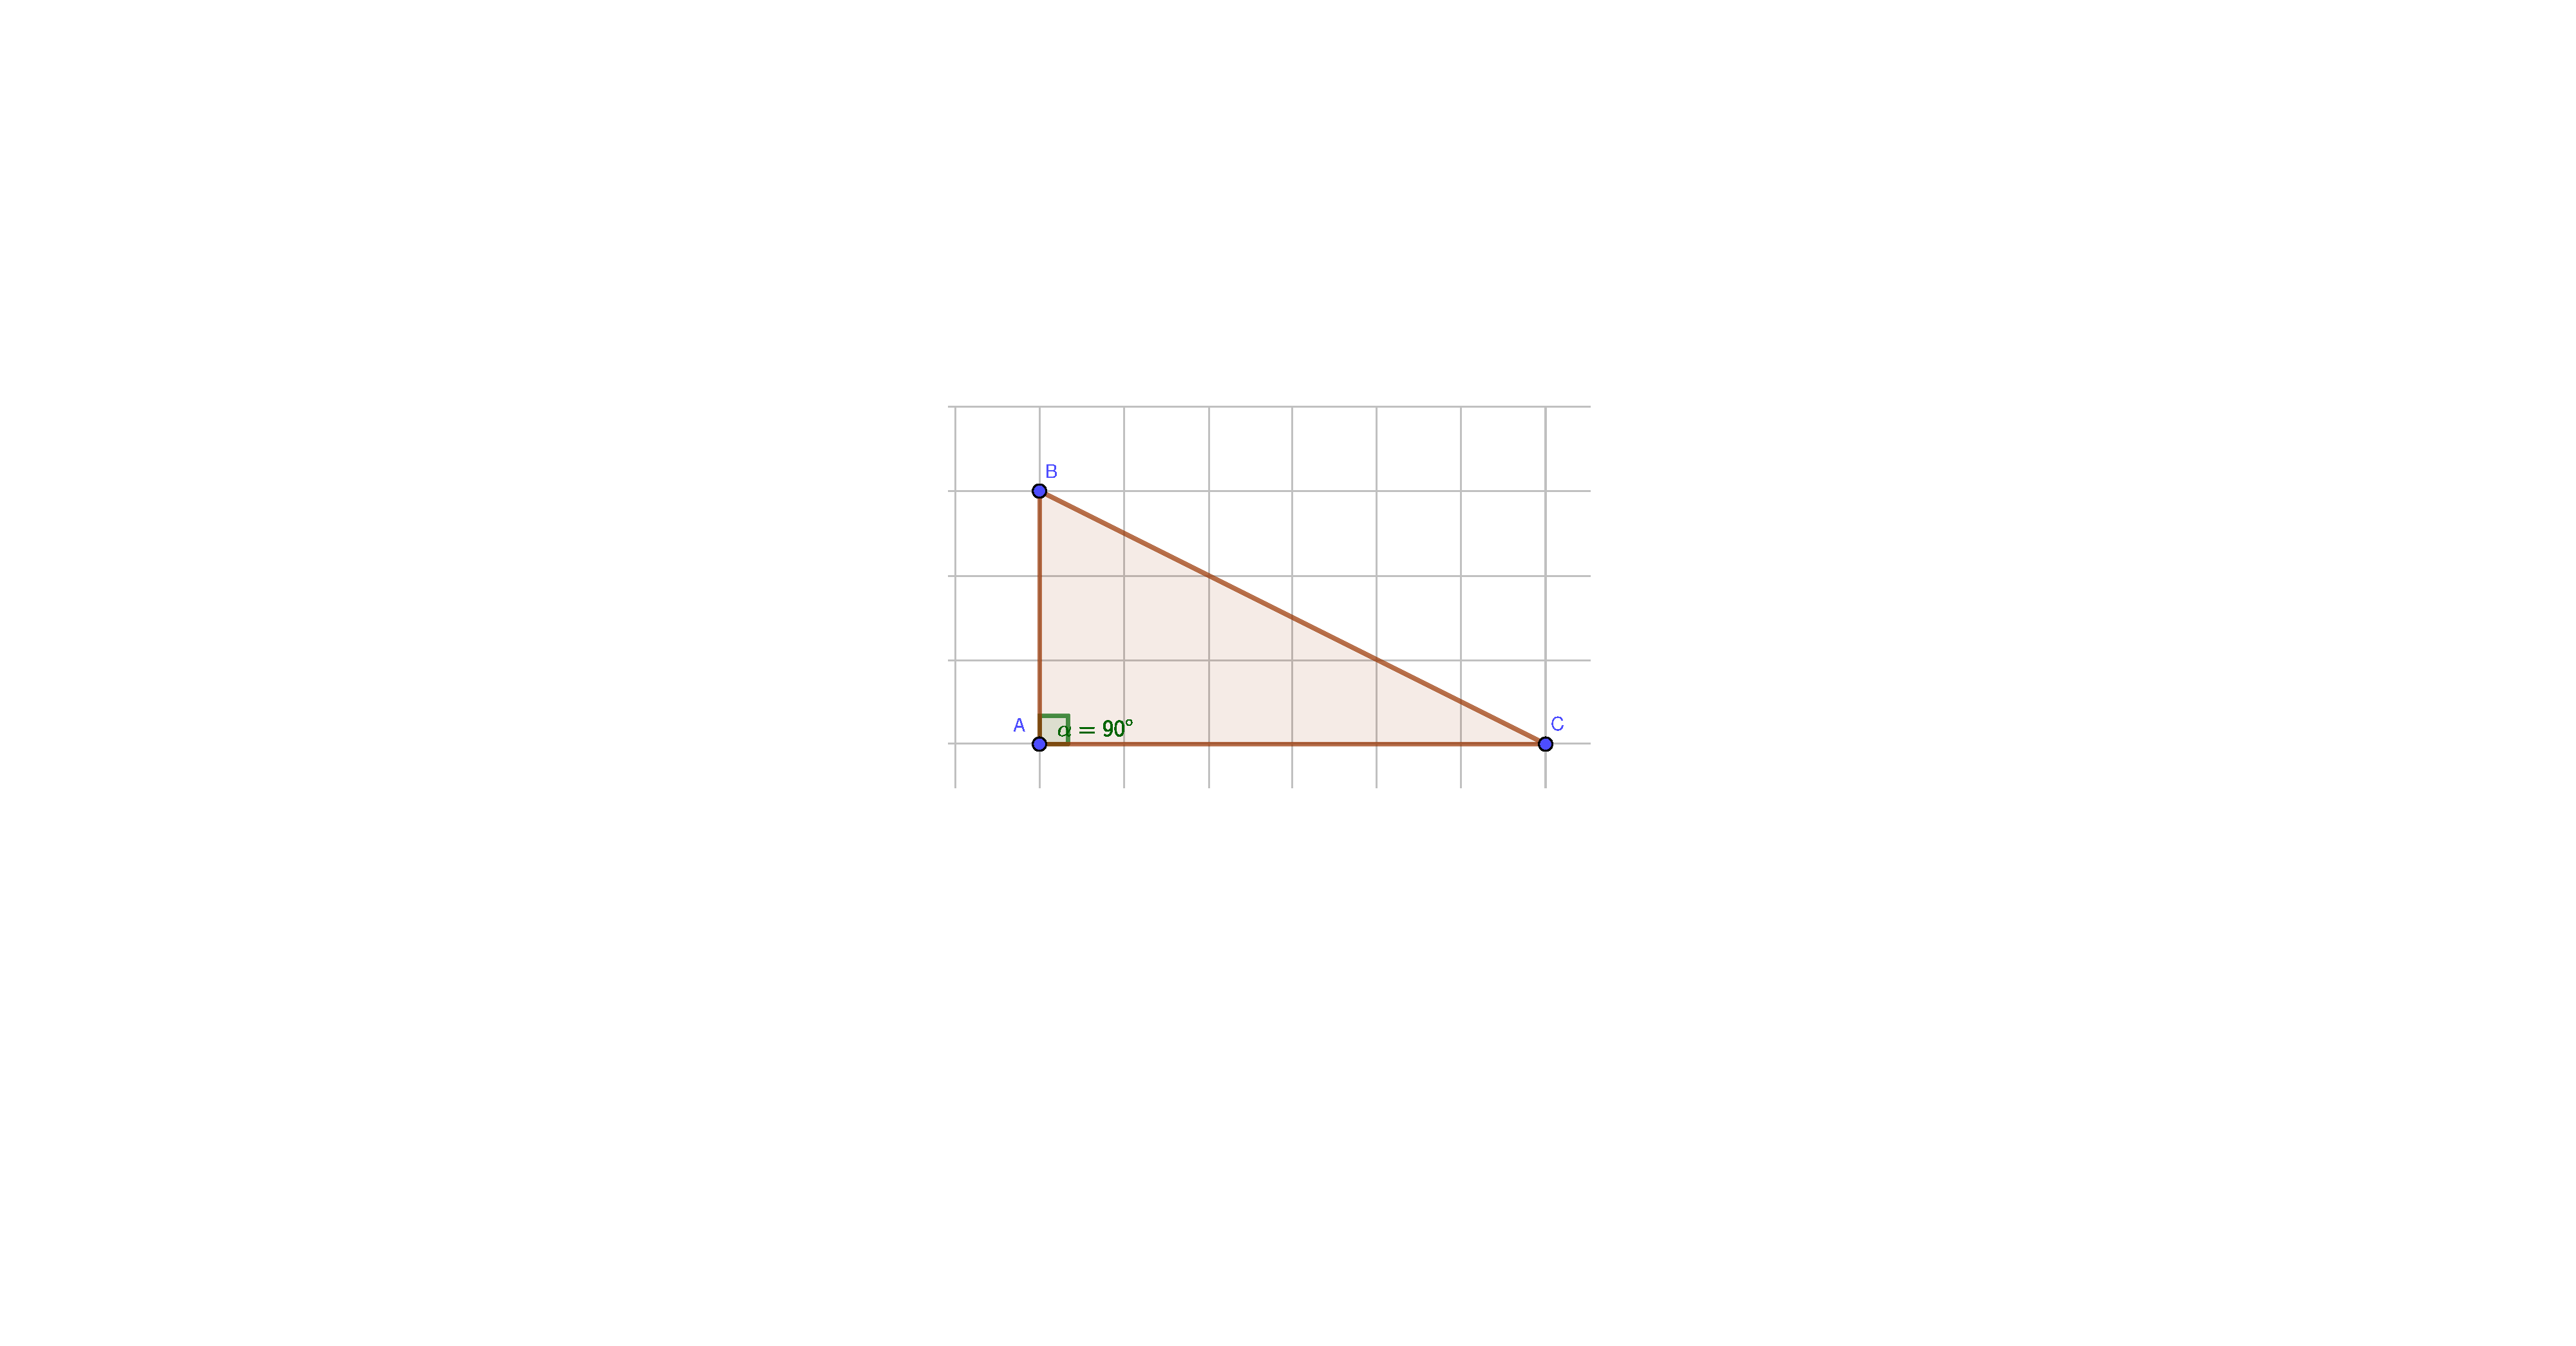
\includegraphics[width=0.6\textwidth]{teor/pravouhly}
    \caption{Pravoúhlý trojúhelník}
    \label{fig:pravouhly_troj}
\end{figure}

Na obrázku~\ref{fig:pravouhly_troj} je vidět pravoúhlý trojúhelník, jehož pravý úhel je označen $\alpha$.

\subsection{Rovnoběžnost}
Přímky jsou na sebe rovnoběžné, pokud se nikdy nepotkají. Úsečky jsou na sebe rovnoběžné, pokud se jimi vedené přímky nikdy nepotkají.

\begin{figure}[h]
    \centering
    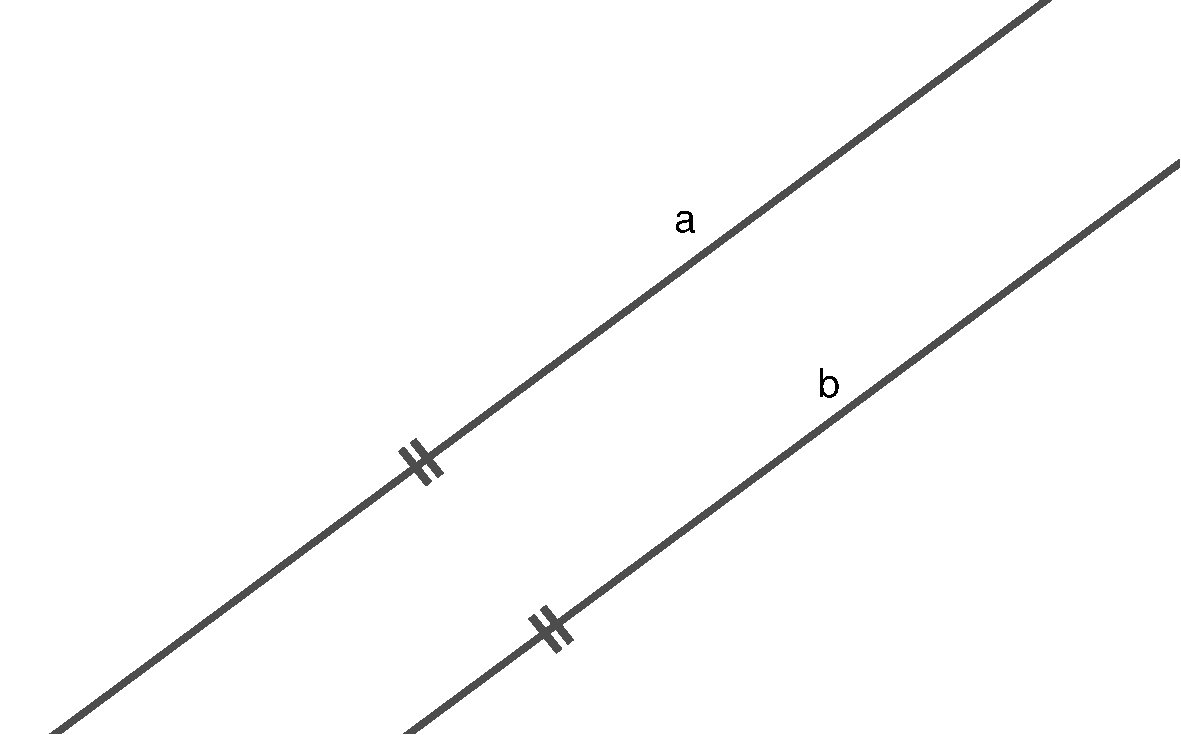
\includegraphics[width=0.6\textwidth]{teor/rovnobezky}
    \caption{2 rovnoběžné přímky}
\end{figure}

\subsection{Krychle}
Krychle je prostorové těleso. Také se nazývá kostka.

\subsubsection{Vrcholy}
Vrcholy krychle jsou body, které jsou v jejích rozích. Krychle jich má 8.

\subsubsection{Hrany}
Hrany jsou čáry, které spojují vrcholy. Krychle jich má 12.

\subsubsection{Stěny}
Stěny jsou čtverce tvořené 4 vrcholy krychle. Krychle jich má 6.

\subsubsection{Povrch}
Povrch krychle je součet obsahů jejích stěn, neboli 6krát obsah jedné stěny. Měří se v jednotkách obsahu.

Na obrázku~\ref{fig:krychle} je krychle, na které jsou červeně vyznačeny vrcholy, modře hrany a zeleně stěny.

\begin{figure}[h]
    \centering
    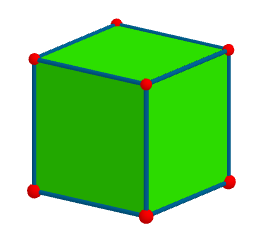
\includegraphics[width=0.6\textwidth]{teor/kostka}
    \caption{Krychle}
    \label{fig:krychle}
\end{figure}


